% This is samplepaper.tex, a sample chapter demonstrating the
% LLNCS macro package for Springer Computer Science proceedings;
% Version 2.21 of 2022/01/12
%
\documentclass[runningheads]{llncs}
%
\usepackage[T1]{fontenc}
% T1 fonts will be used to generate the final print and online PDFs,
% so please use T1 fonts in your manuscript whenever possible.
% Other font encondings may result in incorrect characters.
%
\usepackage{graphicx}
% Used for displaying a sample figure. If possible, figure files should
% be included in EPS format.
%
% If you use the hyperref package, please uncomment the following two lines
% to display URLs in blue roman font according to Springer's eBook style:
%\usepackage{color}
%\renewcommand\UrlFont{\color{blue}\rmfamily}
%
\usepackage{xcolor}
\usepackage{amsfonts}
\usepackage{mathtools}
\usepackage{hyperref}
\usepackage{marginnote}
\usepackage{verbatim}
\usepackage{listings}
\usepackage{amsmath,mathrsfs,amssymb}
\usepackage{multirow}

\newcommand{\term}[1]{\mbox{\texttt{\textbf{#1}}}}
\newcommand{\run}[2]{\term{run}^{#1}\,\left[#2\right]}
\newcommand{\todo}[1]{{\bf\color{red}#1}}
\newcommand{\rel}[3]{{#1}\xrightarrow{#2}{#3}}
\newcommand{\prg}[1]{\mbox{\lstinline|#1|}}
\newcommand{\precprec}{\prec\mathrel{\mkern-5mu}\prec}

\newcommand{\grc}[2]{{#1}\,\left<{#2}\right>}
\newcommand{\java}[1]{\texttt{#1}}
\newcommand{\primi}[1]{\mathbf{#1}}
\newcommand{\cc}[1]{\lfloor{#1}\rfloor}
\sloppy

\lstdefinelanguage{ocanren}{
keywords={run, conde, fresh, let, in, match, with, when, class, type,
object, method, of, rec, repeat, until, while, not, do, done, as, val, inherit,
new, module, sig, deriving, datatype, struct, if, then, else, open, private, virtual, include, success, failure, switch,
true, false, ocanren},
sensitive=true,
commentstyle=\small\itshape\ttfamily,
keywordstyle=\ttfamily\textbf,
identifierstyle=\ttfamily,
basewidth={0.5em,0.5em},
columns=fixed,
mathescape=true,
fontadjust=true,
literate={fun}{{$\lambda$}}1 {->}{{$\to$}}3 {===}{{$\equiv$}}1 {=/=}{{$\not\equiv$}}1 {|>}{{$\triangleright$}}3 {\\/}{{$\vee$}}2 {/\\}{{$\wedge$}}2 {^}{{$\uparrow$}}1
%{[]}{{\texttt|[]|}}1
,
morecomment=[s]{(*}{*)}
}

\lstdefinelanguage{ocaml}{
keywords={type, struct},
sensitive=true,
commentstyle=\small\itshape\ttfamily,
keywordstyle=\ttfamily\textbf,
%keywordstyle=\ttfamily\underbar,
identifierstyle=\ttfamily,
basewidth={0.5em,0.5em},
columns=fixed,
fontadjust=true,
literate={->}{{$\to$}}3 {=>}{{$\Rightarrow$}}3,
morecomment=[s]{(*}{*)}
}

\pagestyle{plain}
\usepackage{lineno}
\linenumbers

\begin{document}
%
\title{Relational Solver for \textsc{Java} Generics Type System}
%
%\titlerunning{Abbreviated paper title}
% If the paper title is too long for the running head, you can set
% an abbreviated paper title here
%
\author{
  Peter Lozov\inst{1}\orcidID{0000-0003-3563-2828} \and
  Dmitry Kosarev\inst{1}\orcidID{0000-0002-6773-5322} \and
  Dmitry Ivanov\inst{2}\and
  Dmitry Boulytchev\inst{1}\orcidID{0000-0001-8363-7143}
}
%
\authorrunning{Dmitry Kosarev et al.}
% First names are abbreviated in the running head.
% If there are more than two authors, 'et al.' is used.
%
\institute{
Saint-Petersburg State University,\\
Universitetskaya emb., 7-9, 199034, St.Petersburg, Russia\\
\email{lozov.peter@gmail.com},\email{kakadu.hafanana@gmail.com},\email{dboulytchev@math.spbu.ru}\\
Saint-Petersburg,\\
\email{korifey@gmail.com}\\}
%
\maketitle              % typeset the header of the contribution
%
\begin{abstract}
  We present a solver for Java generics type system implemented using relational verifier-to-solver
  approach. The solver finds solutions for a system of subtyping inequations with free variables
  and thus can be used to determine a concrete type satisfying a set of constraints. The
  context of this work is symbolic execution for testing and verification of \textsc{Java} programs.
\keywords{\textsc{Java} generics \and relational programming \and relational solvers.}
\end{abstract}
%
%
%
\section{Introduction}
\label{sec:intro}

\textsc{Java}~\cite{java} is one of the most popular high-level programming languages with millions of developers worldwide~\cite{tiobe} and
thousands of applications written in, including critical ones. There is no surprise that methods, approaches and tools for verification and testing
of \textsc{Java} code is an active research topic with applicable results. One of the most prominent and ambitious method for software testing  which
allows to discover some errors invisible for other methods is \emph{symbolic execution}~\cite{Symbolic}.

Our experience shows that a precise \textsc{Java} generics type solver is a crucial part of symbolic execution engine. In SBST-2022 competition~\cite{SBCT} on
automated test generation our symbolic engine UTBotJava~\cite{UTBot} failed to generate tests for several use cases where generic parameters influenced
symbolic execution process, and several generics-related issues are still unresolved\footnote{https://github.com/UnitTestBot/UTBotJava/issues/730, https://github.com/UnitTestBot/UTBotJava/issues/1994, https://github.com/UnitTestBot/UTBotJava/issues/924}.

In this paper we consider the problem of solving a system of subtyping inequations for \textsc{Java} generic types with free variables. Using relational programming techniques and
verifier-to-solver approach we come up with a simple and declarative albeit not very efficient solver; then we apply a number of problem-specific optimizations for boosting the performance,
which gives us a solver with a promising efficiency. As subtyping relation in \textsc{Java} with the presence of generics is known to be undecidable~\cite{JGTC} the solver can not be total;
however due to the completeness of relational search~\cite{certified} it ultimately finds all existing solutions. We do not claim our current result to be an ultimate achievement; 
however is demonstrates pretty well the advantages and caveats of relational programming approach we investigate.


\begin{comment}
so this paper additionally addresses the problem of developing type solver applicable for accurate symbolic execution.

Java type solver is important because it helps in resolving the types of variables and expressions in a Java program during compilation. This is necessary because Java is a strongly-typed language, meaning that every variable, expression, and function must be explicitly declared with a specific data type. 

Without a type solver, it would be difficult for the compiler to determine the type of a variable or expression, leading to errors and bugs in the program. The type solver helps to ensure that the program is type-safe, meaning that all data types are used correctly and consistently throughout the program.

Java type solver plays a crucial role in static source code analysis. Static analysis is the process of analyzing source code without executing it. It is an important technique to identify potential problems or defects in the code before it is deployed or tested.

In static source code analysis, the type solver is used to resolve the types of variables and expressions in the code. By resolving the types, static analysis tools can perform a more accurate analysis of the code. The type solver helps to identify issues such as type mismatches, incorrect use of variables, and inconsistent data types.

Additionally, the type solver can help to improve the accuracy and efficiency of static analysis. By resolving the types at compile-time, the analysis can be performed more quickly and accurately than if the types were resolved at runtime. This can help to identify potential issues earlier in the development process, saving time and resources.

Overall, the Java type solver is an important tool for static source code analysis. It helps to ensure the correctness and efficiency of the analysis, and can help to identify potential issues earlier in the development process.
\end{comment}

\section{Relational Programming, Verifiers, and Solvers}
\label{sec:rel}

%The implementation of our layout synthesizer employs the techniques of relational programming. Here
%we briefly recollect what relational programming is and how the tools we use work.

Relational programming~\cite{TRS} is an approach based on the idea of describing programs as
relations. It can be considered as a branch of logic programming in which the use of
all non-relational constructs (side-effects, extra-logical features) is discouraged. In a
narrow sense relational programming amounts to writing programs in \textsc{miniKanren}~--- a
specifically designed for this purpose embedded DSL. Initially developed for \textsc{Scheme}/\textsc{Racket}
\textsc{miniKanren} later was ported for dozens of host languages\footnote{http://minikanren.org/\#implementations}.
We, specifically, use a strongly-typed \textsc{miniKanren} implementation for \textsc{OCaml}~\cite{ocaml}, called \textsc{OCanren}~\cite{OCanren}.
\textsc{miniKanren} uses the same theory of Horn clauses as \textsc{Prolog} but with a different
concrete syntax with explicit unification, conjunction, disjunction and fresh variable introduction, and
employs a different \emph{interleaving} search strategy~\cite{interleaving}, which is known to be complete~\cite{certified}.
Besides unification with occurs-check, enabled by default, \textsc{miniKanren} can be equipped with other
basic constraints like disequality constraint~\cite{disuni}, finite-domain constraints~\cite{cKanren}, or
constructs of nominal logic~\cite{aKanren}.

In the context of our work the most valuable property of \textsc{miniKanren} is its capability of expressing \emph{reverse computations}.
It is well-known~\cite{SemanticsModifiers,SemanticsModifiers1} that some complicated programs can be constructed as
a result of inversion of some other, much simpler, programs. The relational nature of \textsc{miniKanren} makes
inverse computations particularly easy, which opens a way for relational synthesis~\cite{Untagged,WBirdSeven,PatternMatching}.
More specifically, we use the capability of \textsc{miniKanren} to turn \emph{verifiers} into \emph{solvers}.

It is rather a matter of common knowledge that verifying a solution is, as a rule, much easier than finding one. The idea
of using relational programming is based on the observation that a solver for a certain search problem can be considered as
an inversion of a verifier for the same problem~\cite{searchproblems}. Thus, to solve some problem one just needs (in principle)
to implement a relational verifier for this problem, which is a routine task in the vast majority of cases. We demonstrate
this approach by the following very simple but observable example.

The following relational program in \textsc{miniKanren} implements an addition of two natural numbers in Peano encoding\footnote{It is a
convention in \textsc{miniKanren} programming to superscript relational definitions with ``$^o$''.} (see Fig.~\ref{addition}\ref{rel-add}).
It takes \emph{three} arguments \lstinline|x|, \lstinline|y|, and \lstinline|z|, and performs a
case analysis on the first one using unification ``\lstinline[language=ocanren]|===|''. When
\lstinline|x| is zero, then \lstinline|y| is unified with \lstinline|z|. Otherwise, there is some
\lstinline|x'| which is one less than \lstinline|x|. We recursively calculate the sum of \lstinline|x'| and
\lstinline|y|, setting its value to \lstinline|z'|, and then unify \lstinline|z| with \lstinline|z'| plus one. Thus,
\lstinline[mathescape=true]|add$^o$| implements the relation $\{(x, y, z)\in\mathbb{N}^3\, |\, x+y=z\}$. This relation can
be ``inspected'' by using specific primitive ``\lstinline[language=ocanren]|run$_{\bar{\alpha}}$ {$Q$}|'', where
$Q$~--- some relational expression (\emph{query}), $\bar{\alpha}$~--- a list of fresh \emph{query} variables.
\lstinline[language=ocanren]|run| initiates a search which finds all substitutions for query variables which
make the query to succeed, and return them in a form of a lazy stream. For example, \lstinline[language=ocanren,basicstyle=\small]|run$_\alpha$ {add$^o$ (S O) (S (S O)) $\alpha$}|
will return a single substitution $[\alpha\mapsto \mbox{\lstinline|S (S (S O))|}]$, thus calculating a
sum of \lstinline|S O| (one) and \lstinline|S (S O)| (two). However, at the same time the very same relational
program can be used to decompose a number in all possible summands: \lstinline[language=ocanren,basicstyle=\small]|run$_{\alpha\beta}$ {add$^o$ $\alpha$ $\beta$ (S (S (S O)))}|
will do the job, decomposing \lstinline|S (S (S O))| into all summands and binding them to $\alpha$ and $\beta$ respectively.
Thus, a single relational definition can be run in various ``directions'', solving various search problems.

\begin{figure}[t]
  \centering
  \begin{subfigure}[t]{0.4\textwidth}    
\begin{lstlisting}[language=ocanren,basicstyle=\small]
  let rec add$^o$ x y z = ocanren {
    x === O /\ z === y \/
    fresh x', z' in
      x === S x' /\
      z === S z' /\
      add$^o$ x' y z'
  }
\end{lstlisting}
\caption{Relational addition}
\label{rel-add}
  \end{subfigure}
  \hfill
  \begin{subfigure}[t]{0.4\textwidth}
\begin{lstlisting}[language=ocanren,basicstyle=\small]
   let rec add x y =
     match x with
     | O    -> y
     | S x' -> S (add x' y)     
\end{lstlisting}
\vskip12mm
\caption{Functional addition}
\label{fun-add}
  \end{subfigure}
  \vskip5mm
  \caption{Relational vs. functional addition implementation}
  \label{addition}
\end{figure}

Finally, in many cases it is easier to obtain relational specification from functional one. For example,
relational addition can be easily converted from more conventional functional code (see Fig.~\ref{addition}\ref{fun-add}).
For our task we use a tool, called \textsc{noCanren}, to perform \emph{typed relational conversion}\cite{lozov2017typed}, for which its static and dynamic
correctness was proven formally. Thus, our solution is a mixture of a hand-written and converted relational code and, in fact, a few
different solvers.



\section{Java Generics}

Here we briefly describe the relevant subpart of \textsc{Java} type system. All
information in this section is directly derived from the Java Language Specification~\cite{JLS}.
We also refrain from reiterating on the non-generic part of \textsc{Java} type system assuming the reader's familiarity
with the concepts of reference types, arrays, classes, interfaces, and inheritance.

The subsystem we are dealing with contains generic class/interface types, array types,
type variables, null and intersection types:

\[
\begin{array}{rcll}
  \mathscr{T} & = & \alpha^\mathscr{T}_\mathscr{T_\bot}&\mbox{--- type variable}            \\[2mm]
              &   & \bigcap\,\mathscr{T}           &\mbox{--- intersection type}      \\[2mm]
              &   & \grc{C}{\mathscr{T}^*}         &\mbox{--- class or interface type} \\[2mm]
              &   & \mathscr{T}\mbox{\java{[]}}    &\mbox{--- array type}\\[2mm]     
              &   & \primi{null}                   &\mbox{--- null type}\\[2mm]         
\end{array}
\]

Here $\mathscr{T}_\bot$ denotes optional type.

Type variables are bounded in the sense that they always have a certain \emph{upper bound}. This upper
bound can be either specified explicitly or assumed to be \java{java.lang.Object}. In addition
to the upper bound a type variable can be equipped with a \emph{lower bound}. The lower bound can only
be derived implicitly as a result of \emph{capture conversion} (see below). We denote the upper bound of a variable
by  superscript and lower~--- by subscript.

Generic class (or interface) is a class/interface which is equipped with a number of
type parameters. In generic class declaration these parameters can only be type
variables with specified upper bounds. Additionally a number of \emph{direct supertypes} (notation: ``$\prec$'')
can be specified for a generic class/interface:

\[
\grc{C}{\alpha_1^{U_1}\dots \alpha_k^{U_k}}\prec\grc{S_1}{T^1_1\dots T^1_{n_1}}\dots\grc{S_m}{T^m_1\dots T^m_{n_m}}
\]

Here $C$ is the class/interface being declared, $\alpha_i^{U_i}$~--- its generic parameters with upper
bounds, $S_i$~--- its direct supertypes, among which only one type can be a class type, $T^j_l$~--- type
parameters for direct supertypes, which may contain the occurences of $\alpha_i$; note: neither of $T^j_l$ can be
an intersection type.

Type variables in scopes of their declarations behave like regular types; the scope of a type variable is
determined by the position of its introduction (either generic class/interface or generic method). It
is unclear what is the scope of type variables introduced implicitly as a result of capture
conversion, but this might be irrelevant to the problem we are dealing with.

Intersection types can not be declared explicitly; the only positions in which they can be specified are
upper bounds of type parameters in generic class/interface declarations. However intersection types can be derived
as a result of capture conversion.

Null type is an artificial transparent type with no explicit representation. It is assumed to be a subtype for
every other reference type.

Besides regular types generic classes can be applied to \emph{wildcard types}. A wildcard is an anonymous
type variable (notation: ``\java{?}'') equipped, as a regular type variable, with upper bound and optional lower bound
neither of which can be of intersection type. If no upper bound is specified explicitly then \java{java.lang.Object} is implicitly assumed.
It is important that wildcards can not be used to parameterize direct supertypes in generic class/interface declarations.
Array types can not be directly parameterized by wildcards.

To establish the subtyping relation (denotation: ``$\precprec$'') between types parameterized by wildcards two additional
notions are introduces.

The first one is \emph{contains} relation ``$\supseteq$'' between wildcard types:

\[
\begin{array}{rclcl}
  \java{?}^T&\supseteq&\java{?}^S&,&T\precprec S \\[2mm]
  \java{?}^T&\supseteq&\java{?}&& \\[2mm]
  \java{?}_T&\supseteq&\java{?}_S&,&S\precprec T\\[2mm]
  \java{?}_T&\supseteq&\java{?}&& \\[2mm]
  \java{?}_T&\supseteq&\java{?}^\java{java.lang.Object}&& \\[2mm]
  T&\supseteq& T&&\\[2mm]
  T&\supseteq&\java{?}^T&&\\[2mm]
  T&\supseteq&\java{?}_T&&
\end{array}
\]

This relation in essence is a routine check that a collection of types designated by the ``right'' wildcard type is
contained in a collection of types designated by the ``left'' one.

The second is \emph{capture conversion}. Informally, capture conversion replaces a \emph{nameless} wildcard type
argument by a freshly introduced \emph{named} type variable, thus ``capturing'' some concrete (but statically unknown)
type in a certain context. The motivation for introducing capture conversion is as follows: let us have
some value of a wildcard-parameterized type, say, some collection of type $\grc{Collection}{?}$. Without capture
conversion we would be incapable of dealing with individual elements of this collection (since a wildcard is not a type,
but rather a way to to describe a certain parameterizarion). From a type-theoretic standpoint wildcards intoduce a
certain form of \emph{existential} types with capture conversion serving as a limited form of opening construct~\cite{tapl}.
The detailed theory and the discussion of properties for the wildcard-related fragment of Java Generics type system
can be found in~\cite{wild}.

Capture conversion is defined as follows. Let $\grc{C}{T_1\dots T_k}$ be a generic class/interface type where some of $T_i$ are wildcards. Let
$\beta_i^{U_i}$ be the $i$-th type parameter of $C$'s declaration. Then capture conversion of
$\grc{C}{T_1\dots T_K}$ is the type $\grc{C}{\cc{T_1}\dots \cc{T_k}}$ where the transformation
``$\cc{\bullet}$'' is defined as follows:

\[
\cc{T_i}=\left\{
\begin{array}{lll}  
  \alpha^{U_i[\beta_j\gets \cc{T_j}]}_\primi{null}      &\mbox{if }        T_i=\java{?}  &\mbox{($\alpha$ is a fresh type variable)}\\[5mm]
  \alpha^{B\cap U_i[\beta_j\gets \cc{T_j}]}_\primi{null} &\mbox{if }        T_i=\java{?}^B &\mbox{($\alpha$ is a fresh type variable)}\\[5mm]
  \alpha^{U_i[\beta_j\gets \cc{T_j}]}_B               &\mbox{if }        T_i=\java{?}_B &\mbox{($\alpha$ is a fresh type variable)}\\[5mm]
  T_i                                           &\mbox{otherwise}  & 
\end{array}\right.
\]

Here ``$[\bullet\gets\bullet]$'' denotes a (simultaneous) substitution of type variables with some types. Note, in capture conversion
type parameters of the class under conversion are substituted with the results of the conversion in all bounds.

The subtyping relation ``$\precprec$'', which is the principle notion for the problem we are dealing with, is defined as a reflexive-transitive
closure of the direct supertype relation ``$\prec$''. We already described one case of direct supertyping, the others are as follows:

\[
\begin{array}{rclcl}
  I & \prec & \java{java.lang.Object} &,& \mbox{($I$ is an interface with no}\\
    &       &                         & &\mbox{direct superinterface)}\\[2mm]
  \grc{C}{T_1\dots T_k} & \prec & \grc{C}{S_1\dots S_k} &,& \forall i\, .\, S_i\supseteq T_i\\[2mm]
  \grc{C}{T_1\dots T_k} & \prec & S &,& \grc{C}{\cc{T_1}\dots \cc{T_k}}\prec S\\[2mm]
  \bigcap T_i & \prec & T_i && \\[2mm]
  \alpha^{\bigcap T_i} & \prec & T_i &&\\[2mm]
  T & \prec & \alpha_T && \\[2mm]
  \primi{null} & \prec & T &&\\[2mm]
  T\java{[]} & \prec & S\java{[]} &,& T\prec S\\[2mm]
  \java{java.lang.Object[]} & \prec & \java{java.lang.Object} &&  \\[2mm]
  \java{java.lang.Object[]} & \prec & \java{java.lang.Cloneabe} && \\[2mm]
  \java{java.lang.Object[]} & \prec & \java{java.io.Serializable} &&
\end{array}
\]

Note: the notions ``$\supseteq$'', ``$\prec$'', and ``$\precprec$'' are defined mutually recursive: ``$\precprec$'' is used
to define ``$\supseteq$'', which is used to define ``$\prec$'', which, in turn, is the basic relation to define ``$\precprec$''.

\section{Relational Subtyping Solver}
\label{sec:solver}

The approach of verifier-to-solver conversion relies on the implementation of functional verifier for the problem in question. In our
case such verifier should test if two given ground types are in the subtyping relation. This, in particular, requires implementation
of capture conversion, ``contains'' relation, and direct subtyping verifier. Then a reflexive-transitive closure of the latter has to
be implemented. The functional verifier is then converted into relational form which by construction delivers a subtyping solver for
non-ground types with free variables.

A simple observation, however, makes its obvious that it is in fact much easier to implement reflexive-transitive closure directly
in relational language. Indeed, given relation $R$ its reflexive-transitive $R^*$ closure can be expressed by just

\[
R^*\,(x,\, y) = R\, (x,\, y)\vee x\equiv y\vee\exists\, z\,.\,R\,(x,\,z)\wedge R^*\,(z,\,y)
\]

which can be easily directly encoded in \textsc{OCanren}. However, from the implementation standpoint the application of this technique
imposes a certain problem since ``$\prec$'' and ``$\precprec$'' are mutually recursive, and we expect ``$\prec$'' to be obtained as a
result of relational conversion of functional implementation.

We discuss now the implementation of functional verifier. We do not present the code right here for space considerations but provide
a link\footnote{https://github.com/dboulytchev/JGS/blob/main/src/JGS.ml} to a complete commented source code. The verifier is
implemented in \textsc{OCaml} in a rather direct manner: we encode types as data structures of certain types and give a
direct implementation for all components of subtyping relation except the transitive closure. All these definitions are ``wrapped'' in a
functor (an \textsc{OCaml} module parameterized by a module) which takes \emph{class table} as a parameter. The class table
contains the definitions of relevant set of classes with their direct supertyping encoding, description of their type parameters, etc.
The concrete contents of the class table is supplied by the symbolic execution engine.

To build a mixture of relationally-converted code and relational implementation of transitive closure we use open recursion: the functional
implementation of direct supertyping relation ``$\prec$'' is parameterized by subtyping relation  ``$\precprec$''. In functional implementation
the knot is tied not by transitive closure of ``$\prec$'' but by ``$\prec$'' itself:

\begin{lstlisting}[language=ocanren,mathescape=true]
  let rec ($\precprec$) ta tb = ta $\prec$ tb 
  and ($\prec$) ta tb     = Verify.($\prec$) ($\precprec$) ta tb
\end{lstlisting}

Here ``\lstinline|Verify|'' is a module acquired by an instantiation of the verifier for a simple hand-written testing class table.
Thus, functional verifier can only check the subtyping of types no more then two ``steps'' away from each other.

The next step is applying relational conversion for this functional verifier. For technical reasons this requires a mild
``massaging'' of initial \textsc{OCaml} implementation: arrays (more efficient in functional world) have to be replaced
with lists, and some changes have to be made in order to compensate for the incompleteness of current relational
conversion implementation. Again, we do not show the code here, but provide a link to a complete implementation\footnote{https://github.com/Lozov-Petr/JGS/blob/noCanren/src/JGS.noc.ml}.
After the relational conversion and the parameterization of verifier functor with a classtable a proper recursive knot is tied by a transitive closure of ``$\prec$'', which
completes the construction of the solver. While functional verifier can only work for ground types and return a boolean value, its relational counterpart
searches for all substitution for free variables in incomplete types is order to make them subtype each other.

Upon reading this section one may feel dissatisfaction~--- indeed, the (presumably) most interesting and essential part of the paper discusses nothing more
than some technical issues of encoding the set of formal definitions given earlier. But this is, actually, the very essence of the approach we advocate~---
no specific efforts have to be made in order to come up with domain-specific solver. 



\section{Evaluation}
\label{sec:eval}

We evaluated our solver for a class table containing more than 40000 classes exported by the symbolic execution engine using
nine benchmark queries of various shapes. The results are presented in Fig.~\ref{fig:eval-diagram} in the form of
a bar chart. Here the groups of four bars correspond to different benchmarks, each bar in the group corresponds to a one of
four versions of the solver (left-to-right): with no optimizations, with dynamic transitive closure only, with dynamic class table specialization only,
and with both optimizations enabled.

The benchmark queries are as follows:

\begin{enumerate}
   \item $\alpha$ $\precprec$ \java{java.util.List<Object>}
   \item $\alpha$ $\precprec$ \java{java.util.RandomAccess} $\land$ \\
          $\alpha$ $\precprec$ \java{java.util.AbstractCollection<Object>}
    \item $\alpha$ $\precprec$ \java{java.util.AbstractCollection<Object>} $\land$ \\
          $\alpha$ $\precprec$ \java{java.util.RandomAccess} 
    \item $\alpha$ $\precprec$ \java{java.util.AbstractCollection<Object>} $\land$ \\
          $\alpha$ $\precprec$ \java{java.util.RandomAccess} $\land$ \\
          $\alpha$ $\precprec$ \java{java.util.List<Object>}
    \item \java{javax.management.AttributeList} $\precprec$ $\alpha$
    \item \java{javax.management.AttributeList} $\precprec$ $\alpha$ $\land$ \\
          \java{kotlinx.collections.PersistentVector<Object>} $\precprec$ $\alpha$
    \item \java{kotlinx.collections.PersistentVector<Object>} $\precprec$ $\alpha$ $\land$ \\
          \java{javax.management.AttributeList} $\precprec$ $\alpha$ $\land$ \\
          \java{com.google.common.collect.ImmutableSortedSet<Object>} $\precprec$ $\alpha$
    \item \java{kotlinx.collections.PersistentVector<Object>} $\precprec$ $\alpha$ $\land$ \\
          $\alpha$ $\precprec$ \java{java.util.List<Object>}
    \item $\alpha$ $\precprec$ \java{java.util.List<Object>} $\land$ \\
          \java{kotlinx.collections.PersistentVector<Object>} $\precprec$ $\alpha$
\end{enumerate}


%\begin{itemize}
%    \item The first founr queries are systems of one, two, and three inequations with upper bounds only 1, 2 and 3 upper bounds for standard collection classes and interfaces \java{List}, \java{Abstract%Collection} and \java{RandomAccess}. Note, the 2nd and the 3rd queries are the same 2 upper bounds but with opposite order.
%    \item The next 3 queries are 1, 2 and 3 lower bound for concrete collection classes \java{AttributeList}, \java{PersistentVector} and \java{ImmutableSortedSet}.
%    \item The last 2 queries consist of one upper bound and one lower bound. These bounds the same for both queries but with opposite order.
%\end{itemize}

\begin{figure}[t]
  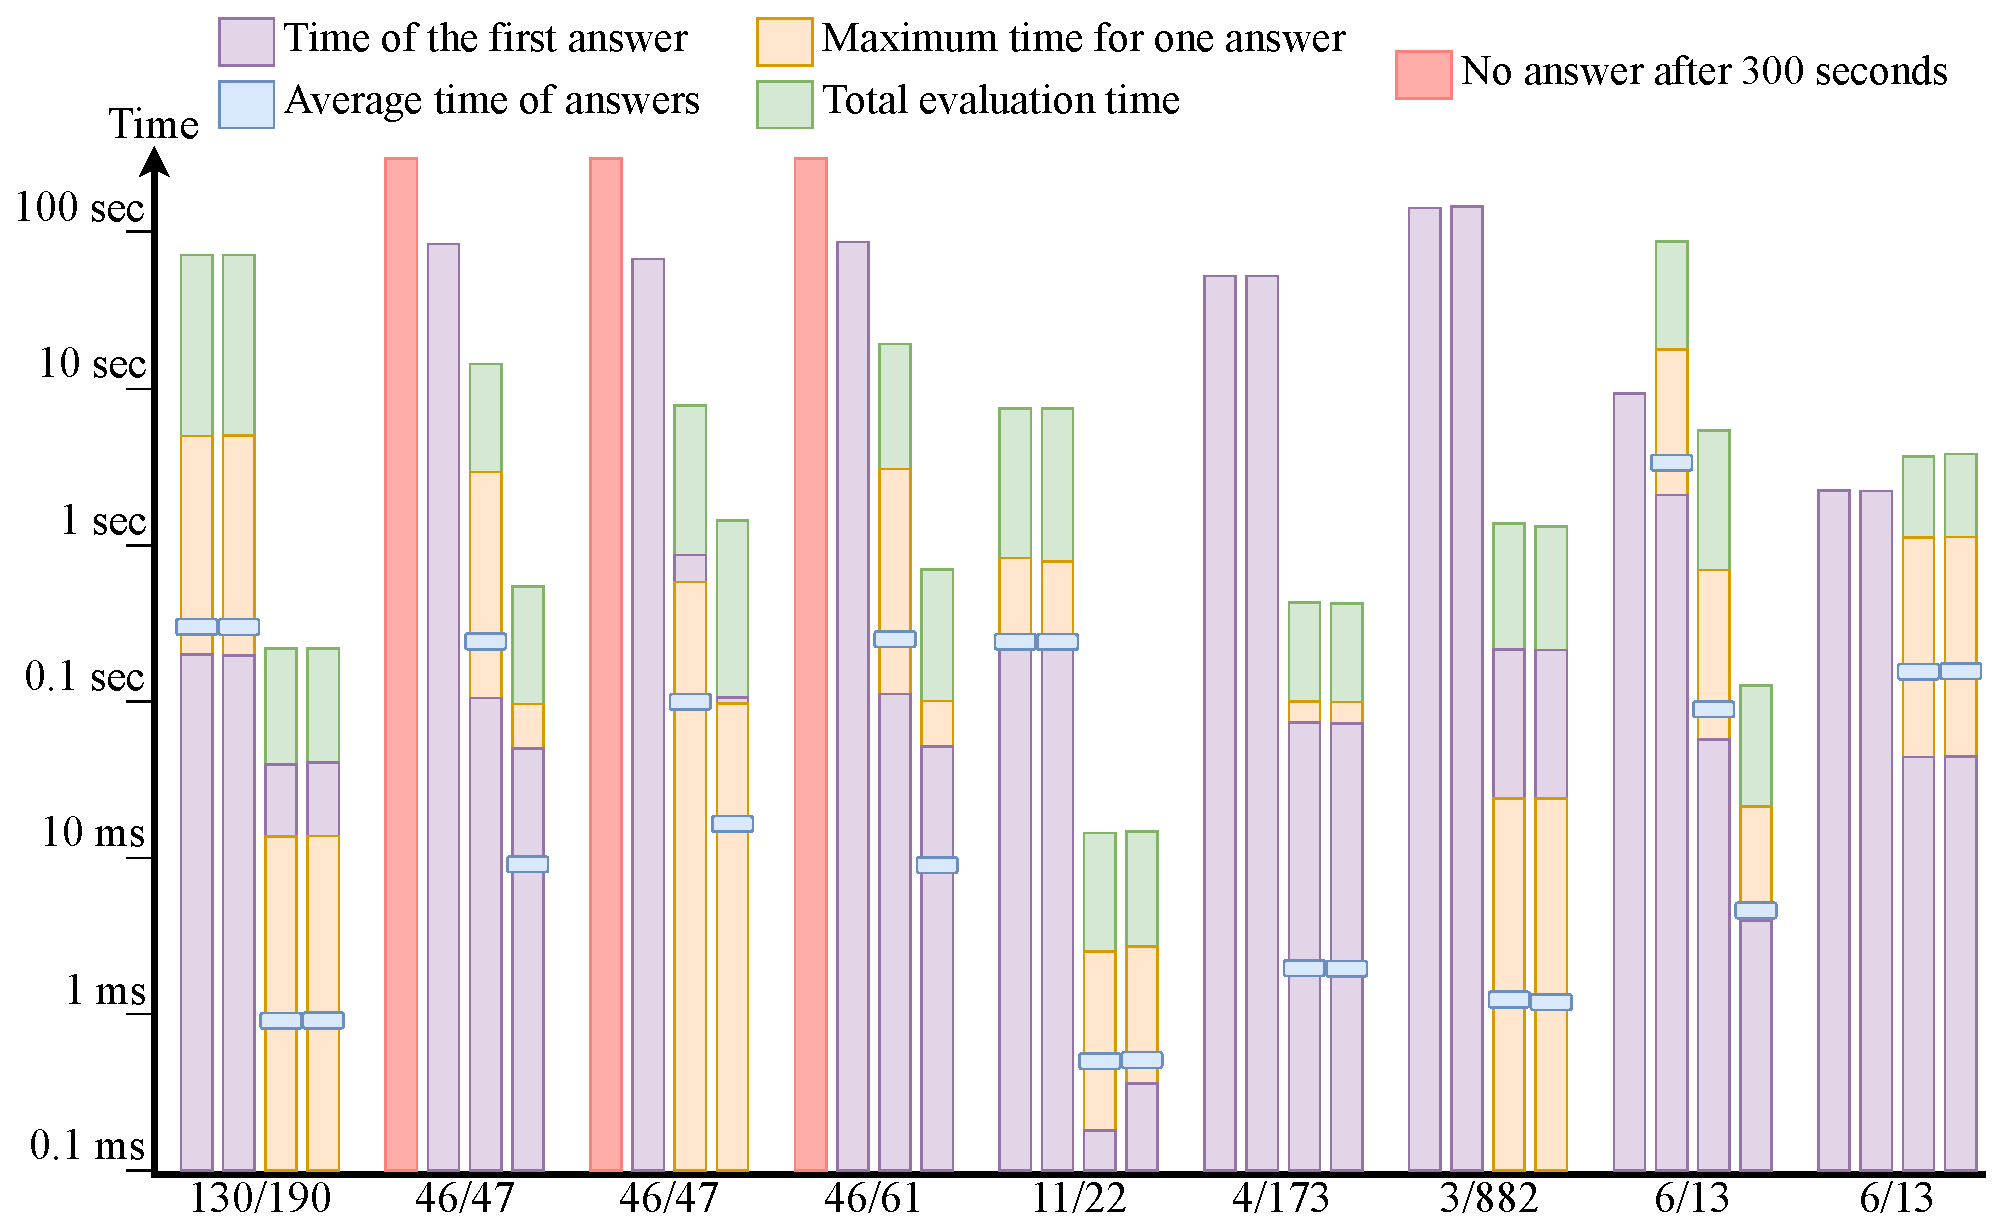
\includegraphics[width=1\textwidth]{eval_diagram.eps}
  \caption{Evaluation results}
  \label{fig:eval-diagram}
\end{figure}

 For each query we evaluated two quantitative measures: the overall number of aswers (shown as a numerator
under corresonding benchmark) and the number of unique answers (shown as a denominator). Also we evaluated four time measures: the time of calculating the first answer (this time includes the time
spent on the pre-calculations required by dynamic table specialization), the maximal time for one answer (not including the first answer time), the average time taken over all answers,
and the total evaluation time. We also limited the evaluation time to 300 seconds; in a few cases we either received only a part of the answers (in this case, only the time for
calculating the first answer is indicated), or we did not receive a single answer (in this case, the red column is shown in the bar chart). All measurements are presented in a logarithmic
scale.

As we can see from the results, dynamic transitive closure in some cases improves the performance by an order of magnitude (if there is an upper bound among the
second and subsequent inequations), dynamic specialization of the table always improves the result by an order of magnitude, but the best performance is achieved when using both optimizations.
It is also noteworthy that the performance of the solver depends on the order of inequations in the query (the benchmarks 3 and 4, 8 and 9 differ only in this aspect). Also, it can be noted that
solving the inequations with lower bounds delivers a large number of duplicate answers.

We can conclude that the optimized version of the solver shows promising performance results, but the problems of performance dependance on the order of bounds and
the presence of duplicates require further research.


\section{Conclusion}
\label{sec:conclusion}

We presented here a first iteration of \textsc{Java} generics type solver implementation using relational verifier-to-solver
conversion technique. While the solver does not demonstrate the desirable performance yet it nevertheless showcases all
major steps, properties, and caveats of the approach we advocate. We consider the development and application of problem-specific
optimizations of the solver as the main direction for future research. Our prior experience shows that such an optimiztions
can boost the performance to the level neccessary to be used as a component in a symbolic execution engine for verification
and testing of real-world \textsc{Java} applications.



%
% ---- Bibliography ----
%
% BibTeX users should specify bibliography style 'splncs04'.
% References will then be sorted and formatted in the correct style.
%
\bibliographystyle{splncs04}
\bibliography{main}
%
\end{document}
